%This whole chapter is my theory chapter.
%Areas to hit are:
% 1. Theoretical approaches to nanoparticles.
%   1.1 Fabrication methods to motivate my coalescence simulations
%   1.2 Properties of interest
%   1.3 Exisitng literature on modelling

% 2. Plasmonics
%   2.1 Phenomenology
%   2.2 Classical description featuring GDM
%   2.3 Quantum mechanical description
%   2.4 Reconcile the two
%   2.5 Plasmon enhanced photocataylysis theory and literature

% 3. Molecular Dynamics
%   3.1 How it works and basic theory to get going. NOT A TEXT BOOK!
%   3.2 How to compute forces e.g., SMATB
%   3.3 Types of dynamics - Melting, Annealing, NVT etc...

% 4. DFT
%   4.1 General introduction hitting the main papers and ideas such as pseudo-potentials etc...
%   4.2 Ground state DFT and what can be computed.
%   4.3 TDDFT and what can be computed
%This is all that needs to be here! 20-30 pages should be the maximum

\noindent\enquote{\itshape If it is not right do not do it; if it is not true do not say it.}\bigbreak

\hfill Marcus Aurelius

\vspace*{0.05\textheight}

In this chapter we introduce and describe the essential physical and numerical theory required to appreciate the methods introduced in Chapter \ref{c:Methods} and the results presented and discussed in Chapters \ref{c:Sapphire}-\ref{c:Water}. We shall introduce and describe pedagogically the realm of nano-science this work concerns itself with; the origins of localised surface plasmons as a collective phenomenom; and how these two components together are utilised to induce photo-catalytic acceleration of specific chemical processes.


\section{Nanoalloys}
\label{sec:NAs_Theory}
\subsection{Morphology}
\label{sec:morph}
A remarkable spillover from academia to industry has long since occurred at the nanoscale. Where once nanoscience was purely the domain of the research scientist - politicians, economists, business leaders, and captains of industry have identified the nanoscale as being an area of profound public interest both now and in the future. In particular, the nanoparticle has become a cornerstone for the most tangible applications of nanoscience today, with uses ranging from the catalysis of chemical reactions to involvement in targeted cancer therapies \cite{doi:10.1021/cr040090g,Fra_Ricardo_Review,ZALESKAMEDYNSKA201680}.

In this section, we shall present and discuss the principles of nanoscience, the deviation with respect to modelling and consideration relative to bulk systems, and motivate a large component of this research project - the importance of morphological and structural properties when probing nanoparticles.

For the purpose of this document, we shall utilise the definition of Roy Johnston, "... an aggregate of a countable number ($2$ - $10^n$, where n can be as high as $6$ or $7$) of atoms...". There is no pre-requisite for each constituent particle to be identical. Indeed, it is when this notion is relaxed do we begin to enter the beautiful world of nanoalloys.


\begin{figure}
\centering
\begin{subfigure}[b]{0.425\textwidth}
    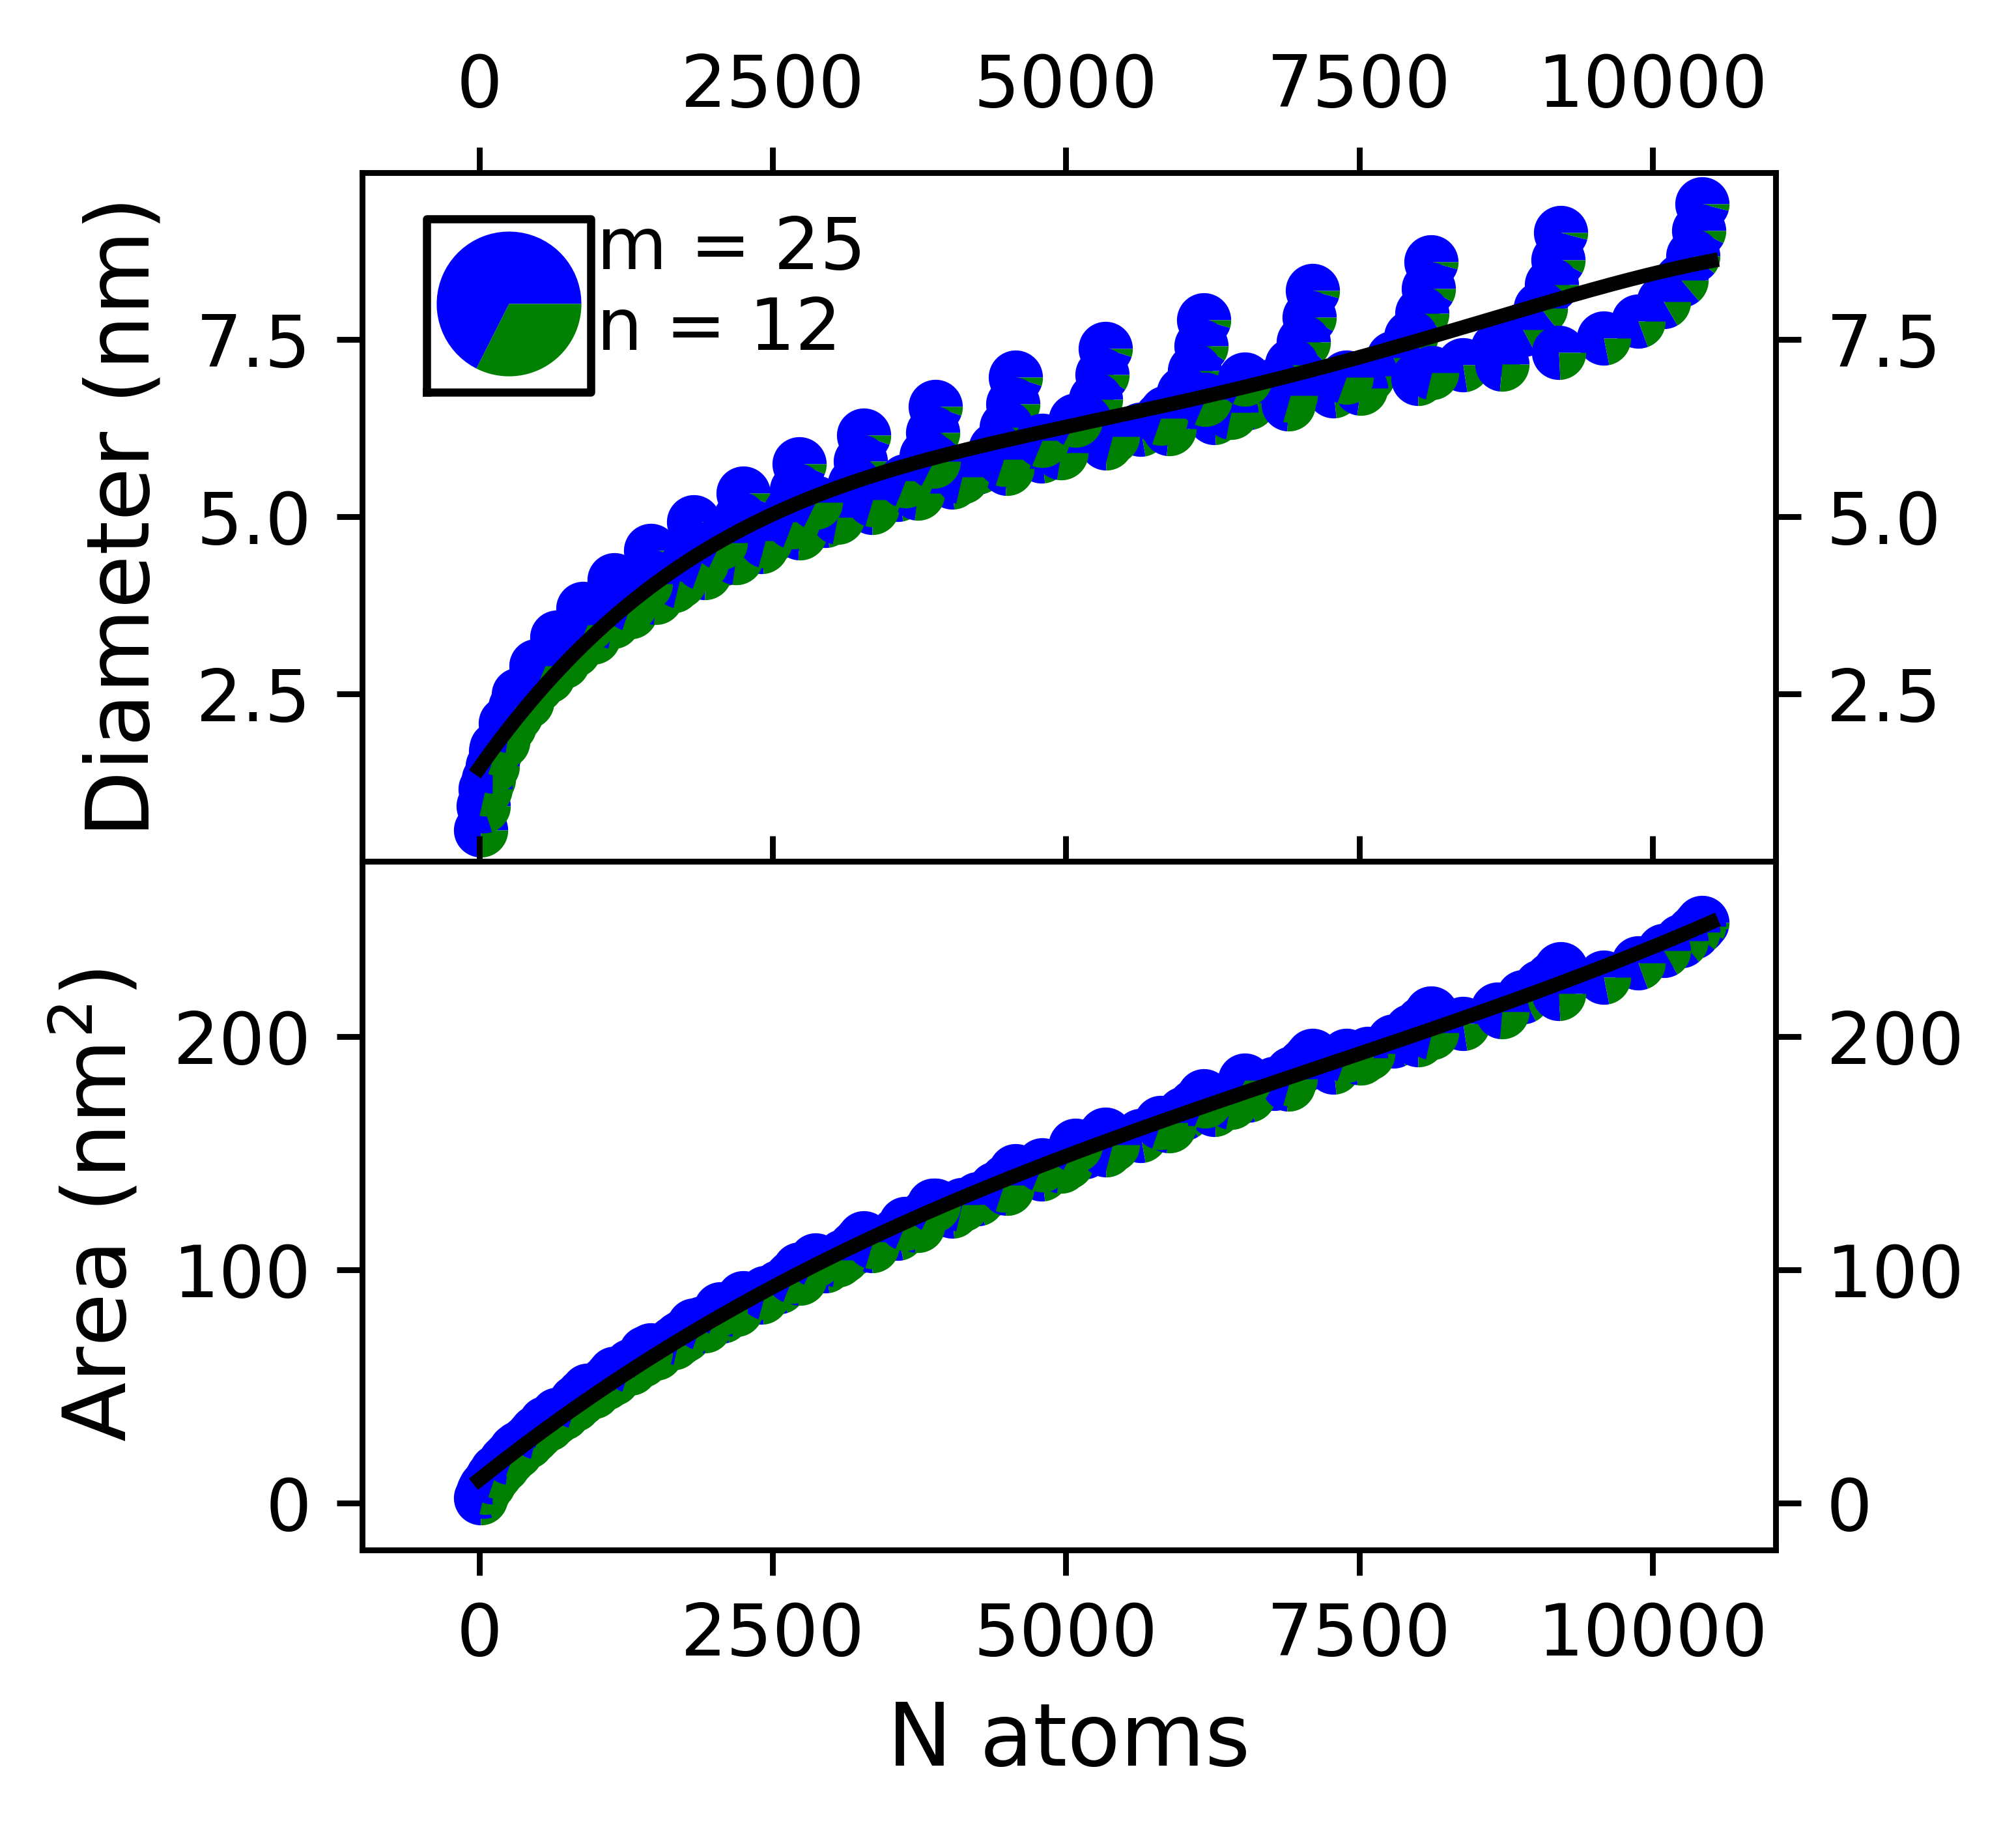
\includegraphics[width=\textwidth]{figures/Theory/To_Size_lin.png}
    \caption{To} 
    \label{Fig:Nps_To}
\end{subfigure}
\begin{subfigure}[b]{0.425\textwidth}
    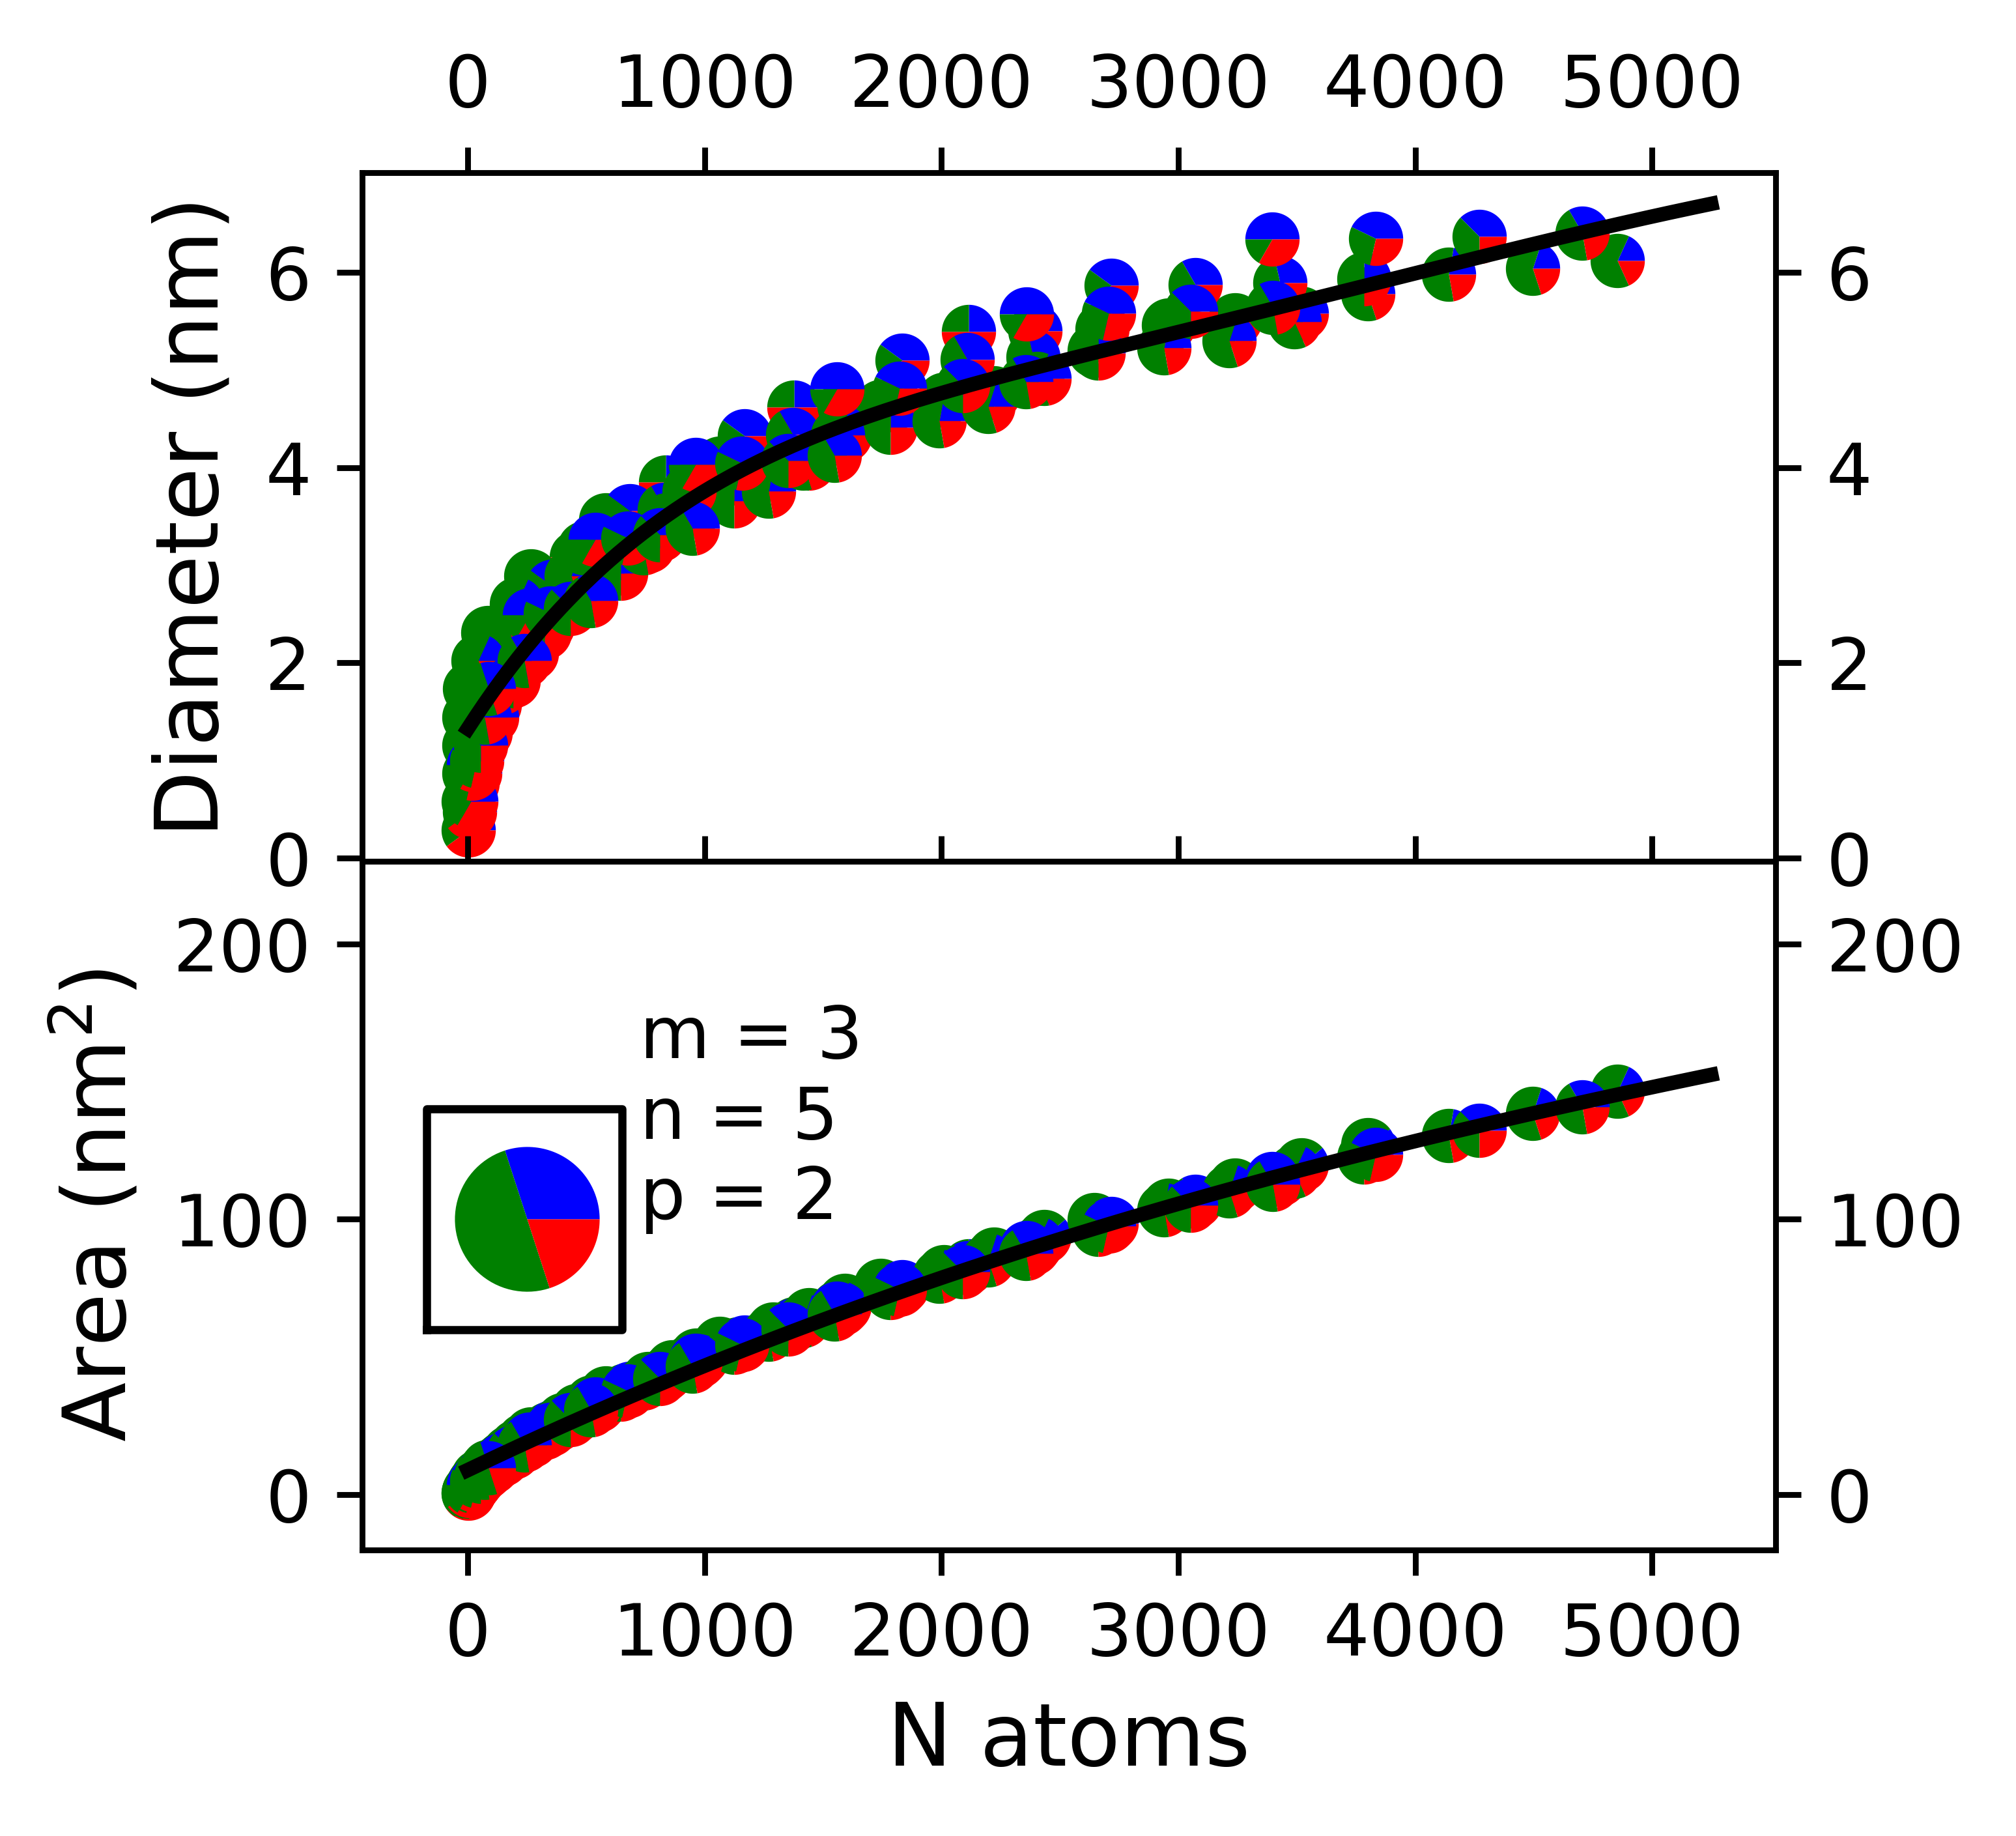
\includegraphics[width=\textwidth]{figures/Theory/MDh_Size_lin.png}
    \caption{MDh}
    \label{Fig:NPs_MDh}
    \end{subfigure}
\begin{subfigure}[b]{0.425\textwidth}
    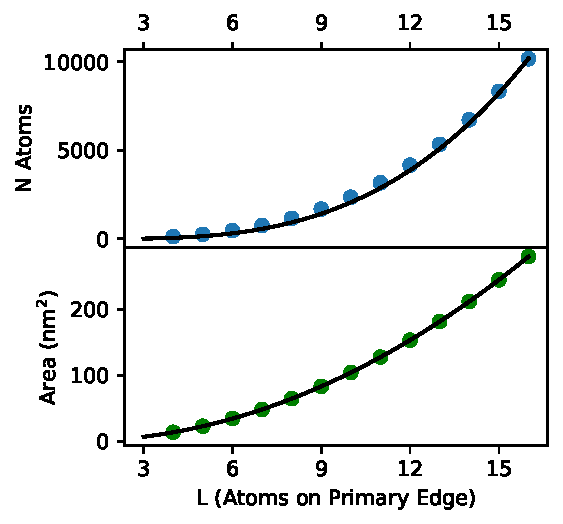
\includegraphics[width=\textwidth]{figures/Theory/Co_Sizes.pdf}
    \caption{Co}
    \label{Fig:NPs_Co}
    \end{subfigure}
\begin{subfigure}[b]{0.425\textwidth}
    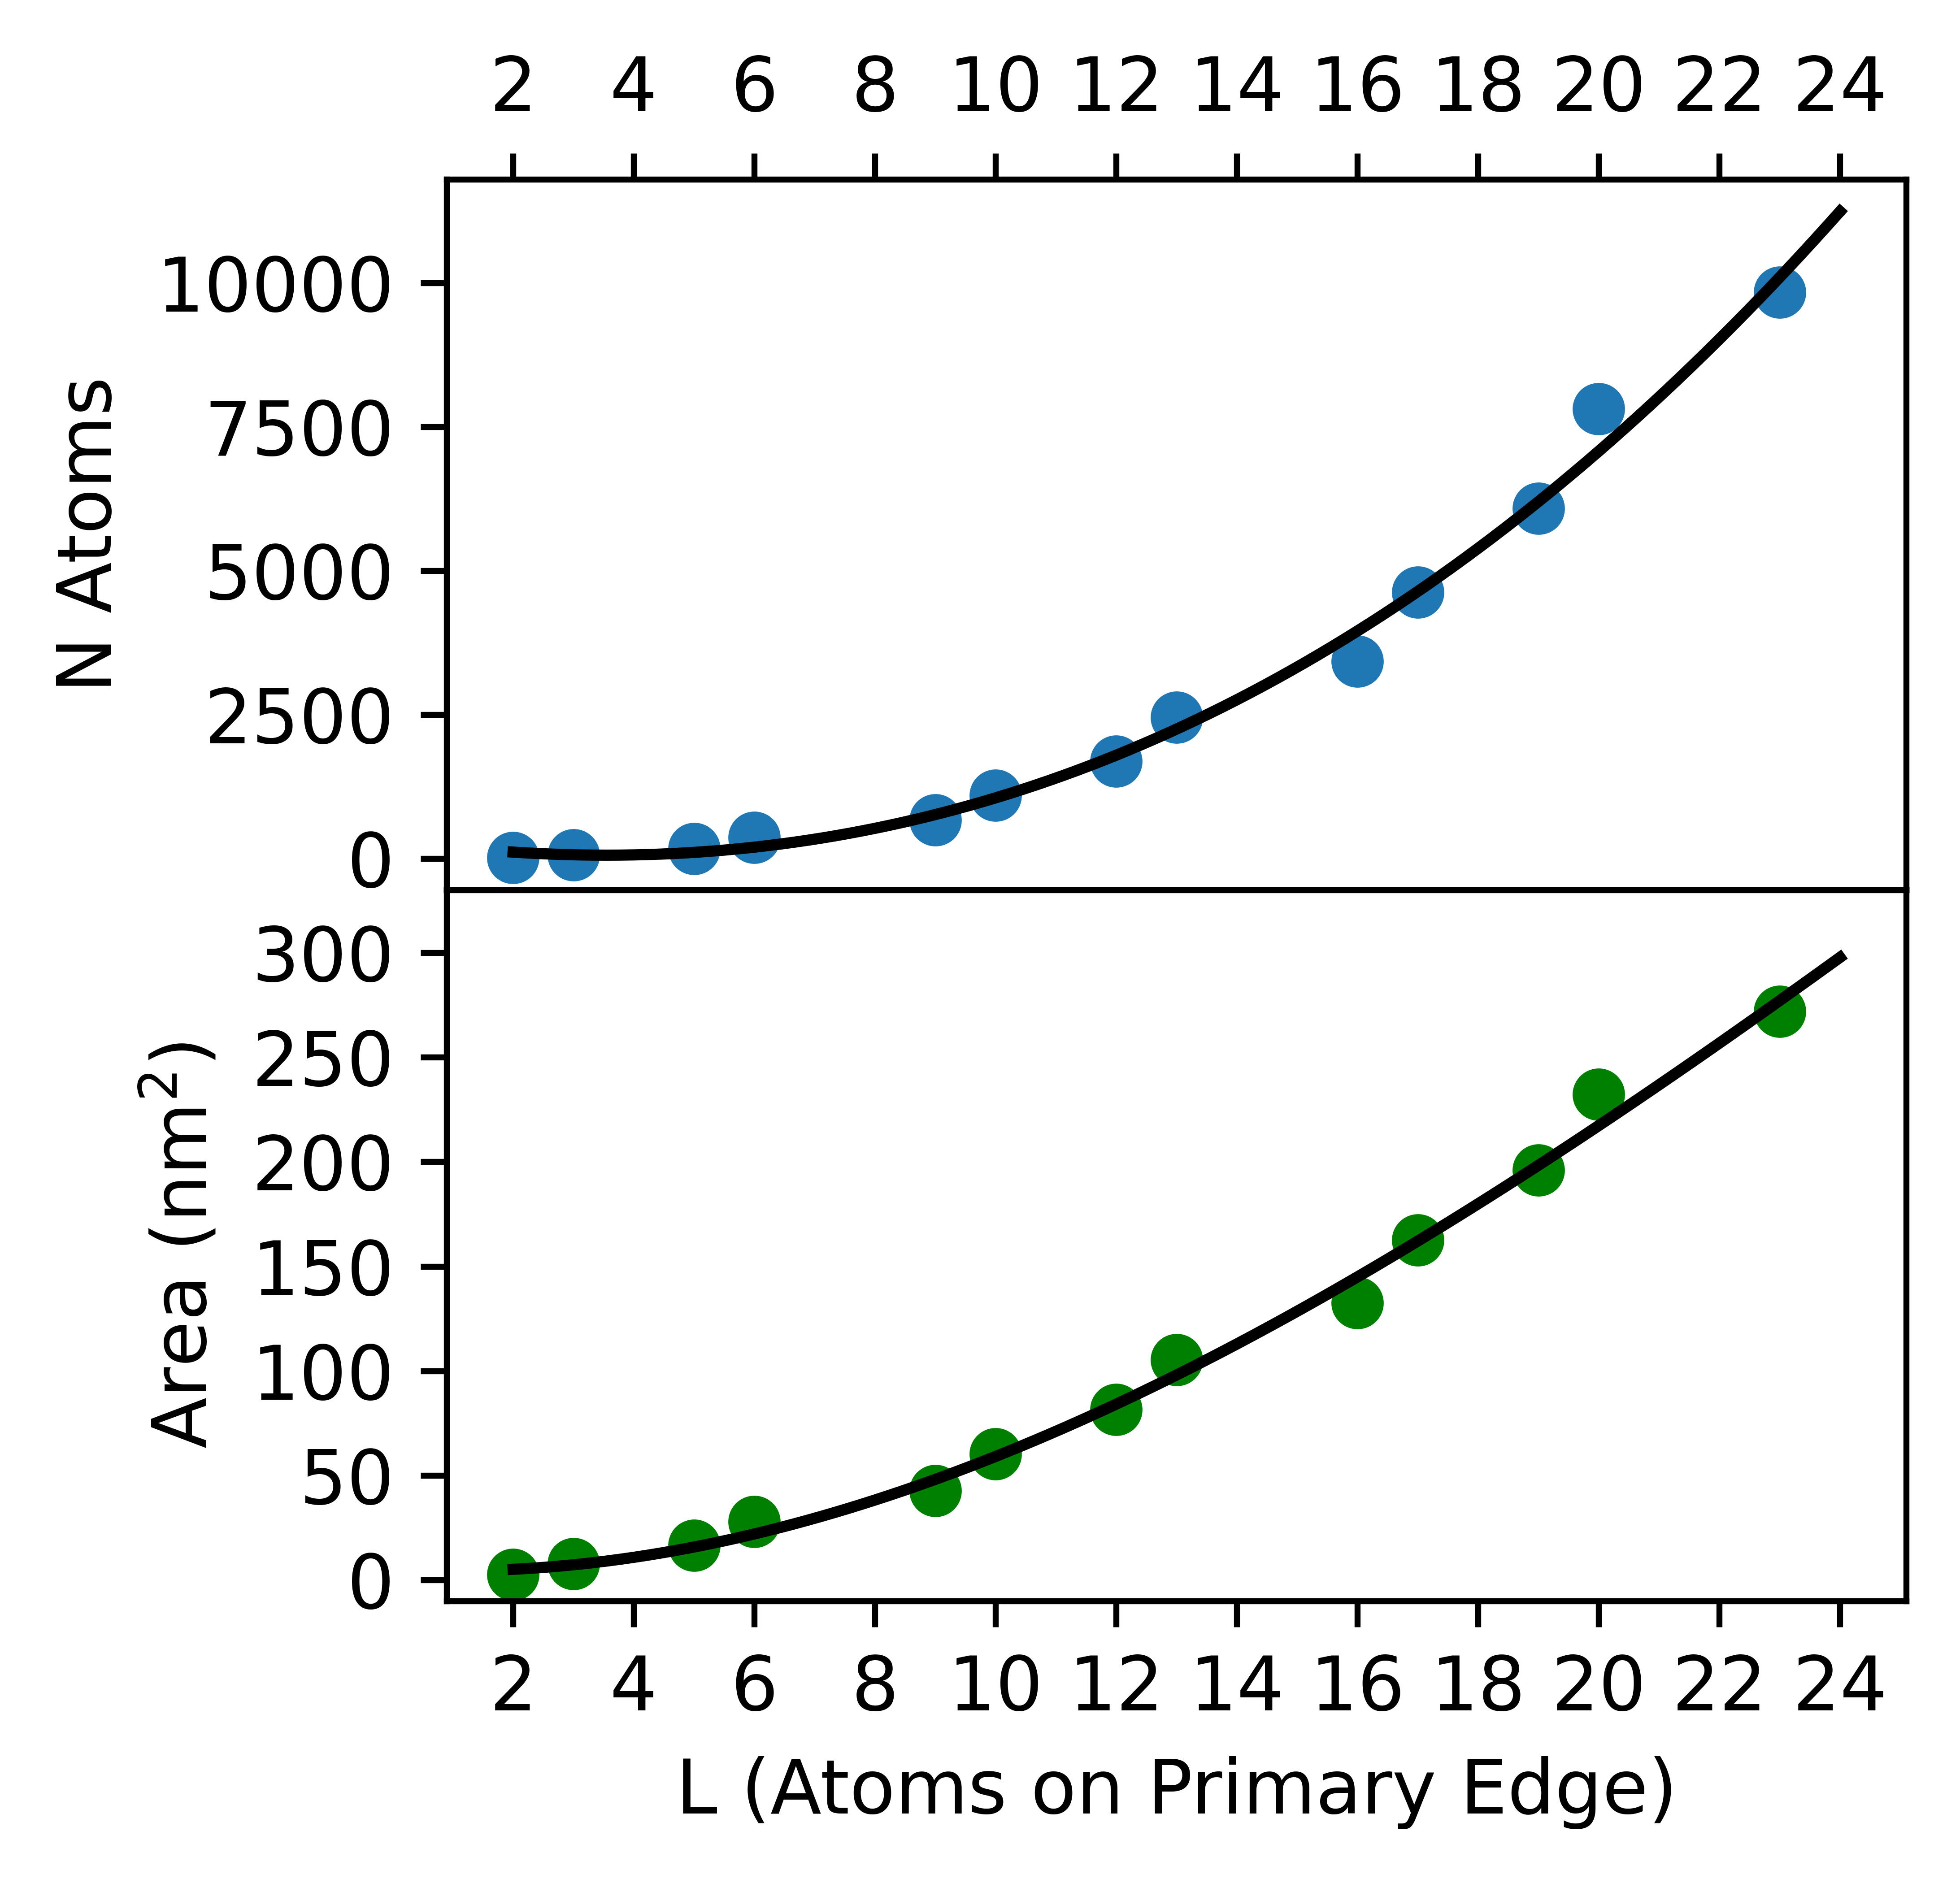
\includegraphics[width=\textwidth]{figures/Theory/Cube_Sizes.png}
    \caption{Cb}
    \label{Fig:NPs_Cb}
    \end{subfigure}
\begin{subfigure}[b]{0.425\textwidth}
    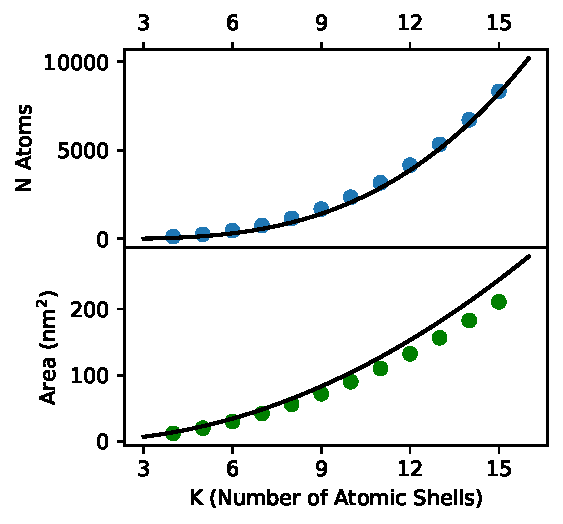
\includegraphics[width=\textwidth]{figures/Theory/Ih_Sizes.pdf}
    \caption{Ih}
    \label{Fig:NPs_Ih}
    \end{subfigure}
\begin{subfigure}[b]{0.425\textwidth}
    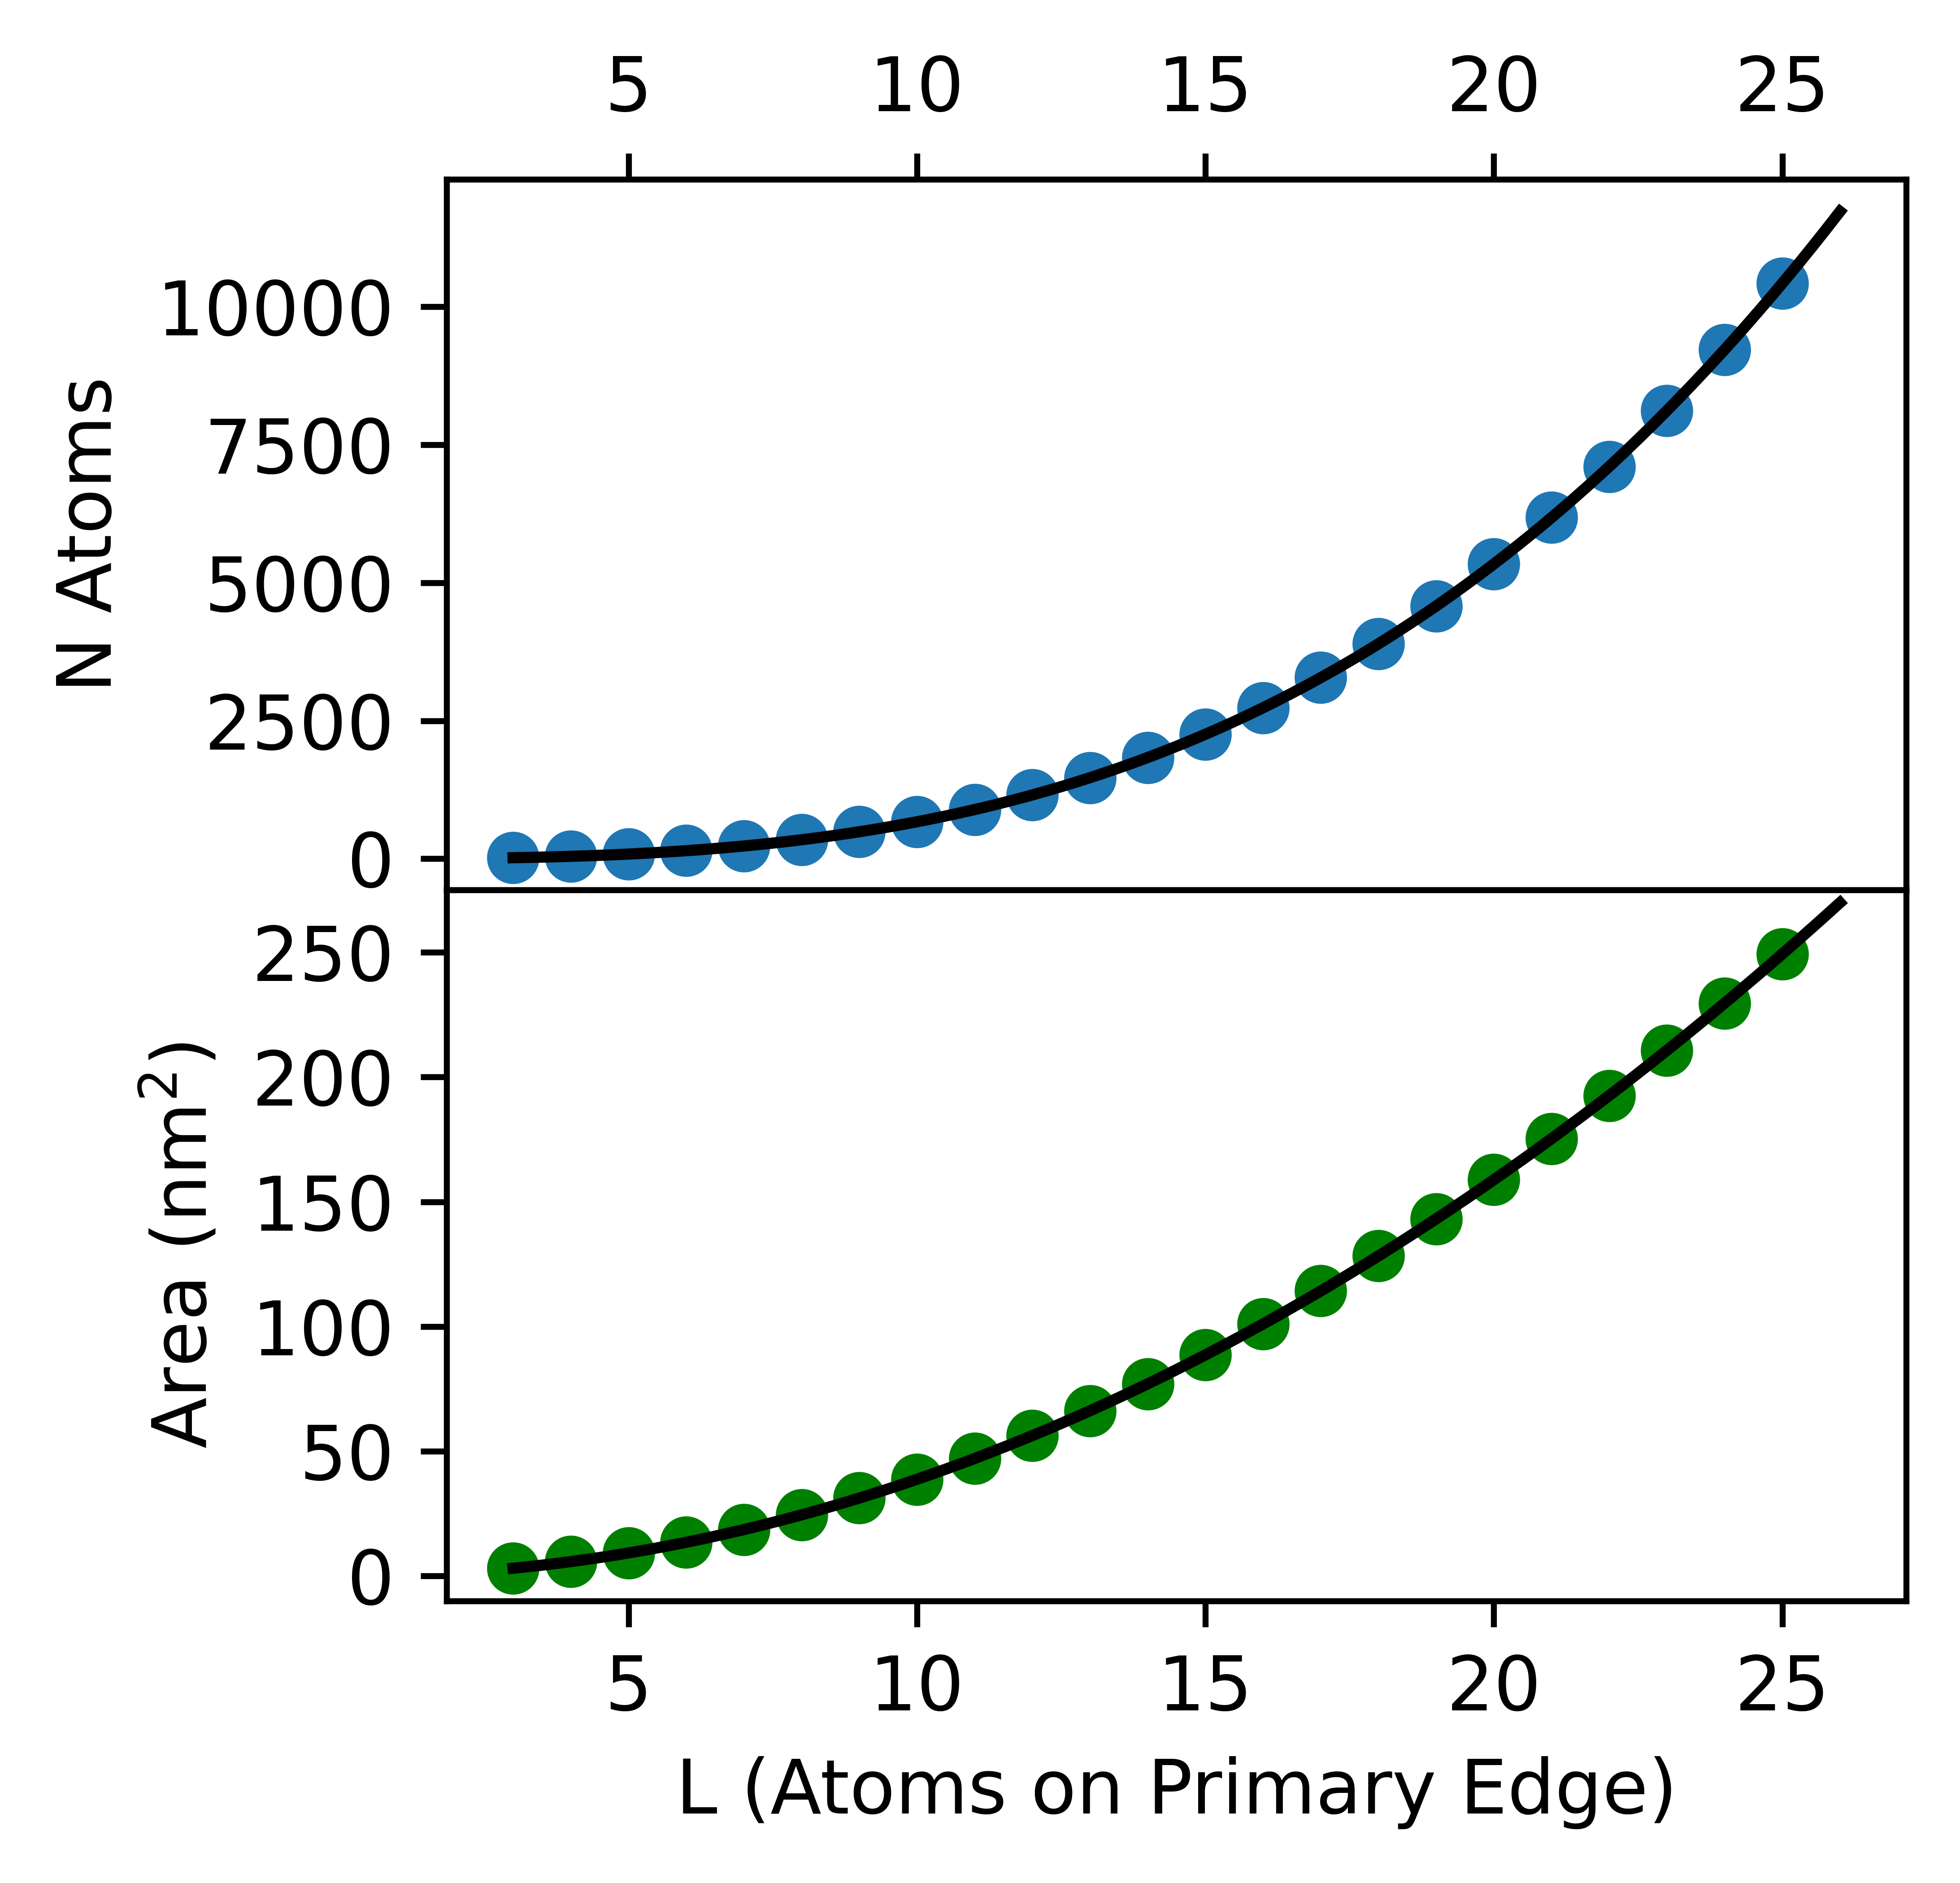
\includegraphics[width=\textwidth]{figures/Theory/Oh_Sizes.png}
    \caption{Oh}
    \label{Fig:NPs_Oh}
    \end{subfigure}
    \caption{Size scaling relations for the discussed NP morphologies. For structures with univariate structural descriptors (\textbf{c, d, e, f}) we plot that descriptor demonstrating the relationship with the number of atoms that polyhedron will contain and the approximate surface area calculated via eqn. \ref{eqn:surf}. Fitting curves demonstrate the relationships stated above. Otherwise (\textbf{a, b}) the number of atoms against the maximal diameter and surface area where the curves are more an aid than a genuine predictive tool. Each marker in (\textbf{a}, \textbf{b}) demonstrates the ratios of the building parameters: m, n, p.}
    \label{Fig:nanoparticles_sizes}
\end{figure}

We present in Figure \ref{Fig:nanoparticles_sizes} the scaling laws at the nanoscale for the regular polyhedra which shall be considered in detail throughout the thesis. These structures are further characterised in List \ref{list:nps}. Most striking are the striations which appear in Figure \ref{Fig:Nps_To} and Figure \ref{Fig:NPs_MDh} which are representative of the style of truncation employed to generate a given structure.

For much of the 20$^{th}$ century, a large component of solid-state physics was dedicated to the consideration and modelling of bulk periodic systems - primarily crystals. This was due to the relative facile nature of describing atomic and electronic properties with respect to regular symmetries. For example, the Bloch theory of electronic structure has been a cornerstone of describing properties such as electrical conductivity and heat capacity. However, when this periodic symmetry is broken in a non-perturbative fashion, the model becomes untenable to describe the physics of the system. 

In few systems is the translational symmetry broken as strongly as it is for finite clusters - with the possible exception of systems such as frustrated glasses. When describing nanoparticles, one must rescind the notion of continuous translational or rotational symmetry, and instead return to more costly, direct methods of describing and predicting properties.

A naive, and yet powerful, approach to describing metallic clusters is to adopt the spherical cluster approximation. This is precisely as it sounds, the cluster may be coarsely approximated to be a uniform sphere which permits the estimation of important geometrical properties such as volume, radius, and surface area. One should not overlook the fact that atoms are already approximated to be spheres and spheres cannot be perfectly tessellated into an arbitrary shape. Consequently, nanometric clusters will be less faithfully described by this model than micrometric or larger. Nonetheless, this approximation unlocks scaling laws and builds the foundation for subsequent models discussed in this thesis.

For a spherical cluster of N atoms of volume $V_a$, the total volume may be crudely approximated as $V_c=NV_a$. By now substituting the spherical radii of atoms, $R_{n}$ and clusters, one arrives at the following scaling relations,

\noindent\begin{minipage}{.25\linewidth}
\centering
\begin{equation}
  R_c = N^{1/3}R_a,
\end{equation}
\end{minipage}%
\begin{minipage}{.25\linewidth}
\begin{equation}
  S_c = N^{2/3}S_a,
\end{equation}
\end{minipage}%
\begin{minipage}{.25\linewidth}
\begin{equation}
  N_s = 4N^{2/3},
  \label{eqn:NA_Surf}
\end{equation}
\end{minipage}%
\begin{minipage}{.25\linewidth}
\begin{equation}
  F_s = 4N^{-1/3},
\end{equation}
\end{minipage}\\

where $S_c$, $N_s$, $F_s$ are respectively the surface area of the cluster, the number of atoms present at the surface, and the fraction of atoms present at the surface. Indeed these are quantities which we will spend much of this thesis in consideration of as we anticipate the majority of the \textit{interesting} chemistry to occur at the surface. 

These quantities become more critical and less trivial as we expand into the domain of nanoalloys for the purposes of catalysis. As motivated earlier, it is the expectation that metals such as Ni, Pd, Pt should be offer chemically active sites - and so determining their contribution to the surface profile is crucial.

We shall provide examples in the existing literature where the discussion regarding the energy and morphologiy of given nanoalloys is spirited, informative, and indeed more exhaustive than we shall be here \cite{PeptidetemplatedAuPtnanoparticlesefficientfunctionalelectrocatalysts,AgAuNanoparticles,AgPdAuPdAuPt,doi:10.1021/cr040090g}. As such, for the purpose of providing the necessary introduction to NA morphology and energy, we shall present only that which is truly necessary. 

We shall principally introduce the taxonomy of NAs from the perspective of the identification of the shape. However, we must also acknowledge the significance that energy plays in the determination of structure. We consider one non-standard contribution to the energetic profile of an NA with respect to the binding energy, $E_{b}$, defined as the total energy minus the excess energy, $E_{Tot} - \Delta E$; where $\Delta E$ is too defined as the excess in energy required to create a finite object constructed from N atoms in the bulk. This quantity is then weighted by the estimate for the number of atoms present at the surface dictated by eqn. \ref{eqn:NA_Surf}.

\begin{equation}
    \Delta E = \frac{E_{Tot} - N\epsilon_{coh}}{N^{2/3}}
    \label{eqn:excessE}
\end{equation}
defines this excess energy quantity, with $\epsilon_{coh}$ being the cohesive energy of the atomic species in the bulk, and all other symbols have their pre-defined meaning.

We shall now acknowledge the highly non-trivial nature of surface energy with respect to finite objects. In principle, this may be simply described as the energy difference between forming a nanostructure, and the alternative of having the same number of atoms in the bulk,

\begin{equation}
    \gamma = \frac{ E_{Tot} - N\epsilon_{coh}}{S_{c}}
    \label{eqn:surf_en}
\end{equation}
where the new quantity $\gamma$ is indeed the surface energy. At first, one may be tempted to assign the area of the NA in the fashion described above. However, to do so is to neglect the contributions made by non-equivalent surface features. For example, two atoms known to be present at the surface may not equally contribute to the total surface area. Nor indeed do two clusters with the same number of surface atoms necessarily have equivalent surface areas due to morphological effects. To approach the issue of interrogating the area of the cluster, we shall begin by introducing the atop generalised coordination number (aGCN) \cite{Calle-Vallejo2014} defined as:
\begin{equation}
    aGCN_{i} = \sum_{j} \frac{CN_{j}}{CN_{max}} \mbox{~~~,}
        \label{eqn:aGCN}
\end{equation}
where $i$ denotes the index of the atom in question, $CN_{j}$ is the coordination number of atom $j$, and with $CN_{max}$ set to 12\footnote{We note, here, that there exist morphologies such as Frank-Kasper polyhedra \cite{https://doi.org/10.1107/S0365110X59001499} which are known to have coordination number as high as 14 \cite{Shoemaker:a25444,NELSON19891,doi:10.1073/pnas.1809655115}. However, given that many of these polyhedra are considered to be cuts of bulk FCC, it is not unreasonable to set 12 as the maximum for the aGCN whilst remaining aware of the existence of additional more highly coordinated structures. Indeed, one could extend such a classification to predict and account for Frank-Kasper polyhedra in future iterations of such work.}, as this is the coordination of an FCC atom in the bulk. We point out that for metallic systems, it seems reasonable to consider the total coordination of each atom, $CN_{j}$, regardless of the difference in electronegativity of the chemical species.

Indeed, the use of the aGCN offers a route to estimate the surface area, beyond, e.g., spherical approximations as the cluster surface area can be well approximated by writing it as a sum over atomic contributions, which are a function of the atomic radius $R_{a}$ weighted with their aGCN. The latter is a measure of how much they are "exposed" \cite{Rossi2020}:
\begin{equation}
  S_{c} = 4 \pi \sum_{i}r^2_{at,i}\left(1 - \frac{aGCN_i}{CN_{max}}  \right)
  \label{eqn:surf}
\end{equation}

Beyond this powerful property of the aGCN, there exists an additional three additional utilities which render this quantity invaluable in the evaluation of arbitrary NAs. First, it has been shown to provide a robust linear relationship with the adsorption energy of small molecules (e.g., O, CO, OH) \cite{Calle2015}; second, the aGCN is able to characterise the MNPs surface sites -- avoiding the basic classification into face, edge, vertex; and finally, one may classify a nanoparticle geometry on the basis of its aGCN-genome \cite{Rossi2019}.
%
 
It is worth noting at this juncture that not only do surface : volume ratios vary profoundly as one deviates from  bulk to finite nanoscale object - but so too do other geometrical and morphological properties. Within bulk systems, one will typically expect uniform crystalline regions exhibiting Face Centred Cubic (FCC) properties, or alternatively Body Centered Cubic (BCC) for some of the transition metals. However, at the nanoscale, one is introduced to the dazzling variety of morphologies available to such clusters. Among these, some of the most common are direct sections of bulk material, such as the icosahedron or decadahedron which are, in a manner of speaking, finite FCC structures. 

\begin{figure}
    \centering
    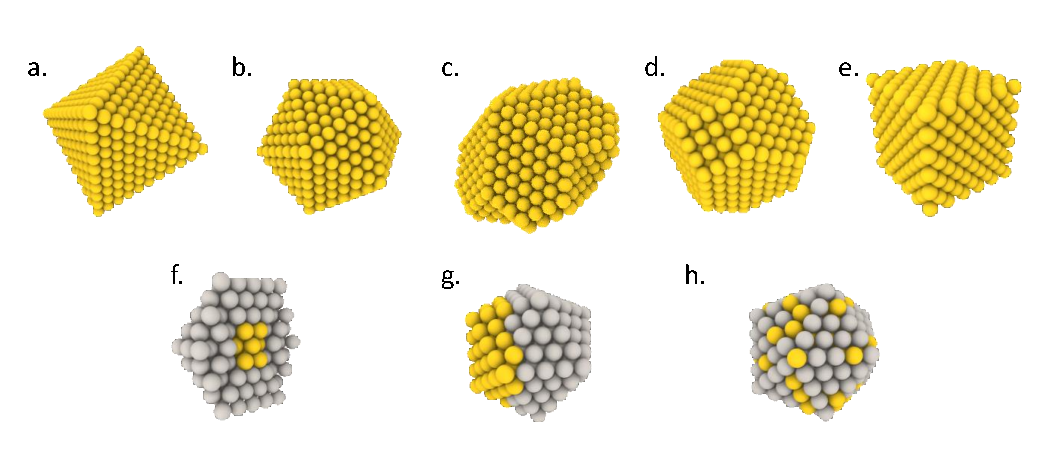
\includegraphics{figures/Theory/Strut_ex.pdf}
    \caption{Common varieties of NA morphology and chemical ordering. Top row is indicative of morphology represented on medium sized ($\sim 1.5$ nm diameter) Au clusters. Bottom row demonstrate common alloying chemical ordering of Au and Pt. Represented Morphologies on the top row are as follows (\textbf{a}) Octahedron (Oh), (\textbf{b}) Icosahedron (Ih), (\textbf{c}) Marks decahedron (MDh), (\textbf{d}) Cuboctahedron (Co), \textbf{e.} cube (Cb). We present on the bottom row are (\textbf{f}) Core-shell (CS), (\textbf{g}) Janus, and (\textbf{h}) Randomly alloyed.
    }
    \label{fig:struts_example}
\end{figure}

Whilst we have not been exhaustive in our presentation of NA morphology in Figure \ref{fig:struts_example}, it is fair to say that it is largely representative of the common regular manifestations of finite size objects. In the following, we shall use the term "Platonic Solid" to describe an object whose edges and faces are all identical. Moreover, when describing the surface area and volume of each structure, we shall assume that the major axis length is unity in an arbitrary basis. We describe these objects below in greater detail, paying attention to specific geometrical properties: 

\begin{itemize}
    \item \textbf{a.} Oh: A platonic solid which may be otherwise considered to be a square-based bi-pyramid. Each face has Miller Indices of (111). Volume and surface area are respectively $\sqrt{2}/3$ and $2\sqrt{3}$.
    \item \textbf{b.} Ih: A platonic solid formed by $20$ tetrahedra sharing a common vertex at the centre. This is the most \textit{spherical} morphology available at this scale, and indeed this feature is why the Ih, and its unit tetrahedron, feature heavily in the following work so that we may work close to the domains of the liquid drop modek and Jellium models which are largely reliant on the notion of sphericity. Each face has Miller Indices of (111). Volume and surface area are respectively $5(3+\sqrt{5})/12$ and $5\sqrt{3}$. Ih are a member of the \textit{magic number} family in that it may be formed by $k$ complete shells where the number of atoms may be exactly computed to be $N_{Ih} = \frac{1}{3} ( 10k^{3} - 15k^{2} - 11k) - 1$. As a final observation regarding the Ih, one may note that nature often favours this particular geometry in that viruses often appear as an Ih, and we as humans are not blind to the beauty of the Ih as many of our modern architectural marvels heavily feature the Ih in subtle to strongly explicit fashions.
    \item \textbf{c.} MDh: The fundamental decahedron (Dh) is formed by the joining of two pentagonal based pyramids at their bases. In general, one may continue to truncate the standard Dh and denote this truncation with three integers ($m$, $n$, $p$) which define the number of atoms along the rectangular (100) Miller Indexed face - edge boundaries and the number of atoms along the re-entrance lines (visible as the top line segment of Figure \ref{fig:struts_example}) on the 5-fold symmetry axis. We construct the MDh specifically by truncating the re-entrances along twin boundaries, where $p>1$. The height, and therefore maximal diameter, is given as $h = m+n+2p -1$, where the surface area is $\frac{5\sqrt{2}}{2} ((m+p-1)(m+3p-1) + 2m) + 5mn$. Indeed, describing the volume is far less trivial and is not presented here.
    \item \textbf{d.} Co: A truncation of the standard Oh described above which results in the creation of 8 (111) Miller indexed faces and 6 perfectly square (100) faces.  Each of the 12 identical vertices share $2$ pf these face types. Volume and surface area are respectively $\frac{5}{3}\sqrt{2}$ and $6+2\sqrt{3}$. As a point of curiosity, the nature of the truncation required to form the Co leads it to join the same morphological family of the Ih in that it follows the same \textit{magic number} law responsible for the Ih.
    \item \textbf{e.} Cb: Possibly the most well-known Platonic solid. Consists of 6 perfectly square (100) Miller Indexed faces. As expected, the volume and surface area are respectively 1 and 6.
    \label{list:nps}
\end{itemize}

Given the vast array of chemical species and the manifold variations on the chemical ordering available at the nanoscale, it should not be a surprise that there exist many fabrication techniques for creating such systems. Each of which will have its own unique utility depending on the desired intent for the system. We shall briefly explain and motivate several techniques which are believed to be pertinent in this line of study and that we shall be attempting to model in Chapter \ref{c:Coal}.

Recent experimental results \cite{Namsoon2021,Kummel2013,Deng2010,Erhart2018} have predicted and observed the formation of a quasi-Janus or of a partial-onion-shell (POS) ordering in AuPt NPs. This may be understood by appealing to the argument of energetic consideration, the species with the greater cohesive energy have the tendency to sink into the structure formed of a less cohesive metal. Moreover, a relaxation of the compressive stress, \textit{i.e.,} local atomic pressure\cite{Taran2020,Bochicchio2013}, may also be a driving force for structural and chemical arrangements. However, these arguments do not elucidate upon the precise atomistic mechanisms responsible for creating such stable or metastable chemical orderings.

\subsection{Nanothermodynamics}
\label{sec:nanotherm}

%In general, just need to capture the key ingredients.
%Can absorb the plasmon stuff into the nanoalloys section.
%
\section{Plasmonics}
\label{sec:plasmons}
\subsection{Origins}
\label{sec:origins_plasmon}
A metal may be modelled to be a plasma in the sense that it is a neutrally charged system consisting of at least one mobile population of charge carriers. Considering a standard metal, the positive ion cores are locked in place, forming a lattice, and valence electrons may be modelled as a gas acting under the influence of the Coulomb potential induced by the lattice of ions. By solving classical equations of motion for a macroscopic electron gas subject to an external field and accounting for both macroscopioc polarisability, and interband transitions by the introduction of additional terms, one may derive an expression for the complex dielectric function of a metal with respect to the plasma frequency. 

\begin{equation}
    \varepsilon(\omega) = \varepsilon_{\infty} - \frac{\omega_{p}^{2}}{ \omega^{2} + i\gamma\omega }.
    \label{eqn:RealDrude}
\end{equation}

Equation \ref{eqn:RealDrude} describes the dielectric behaviour of a conducting medium at frequency $\omega$, $\varepsilon_{\infty}$ is a constant term which may be modified to describe a real metallic system, often in the range $ 1 < \varepsilon_{\infty} < 10$, $\gamma$ is the frequency of electron - electron collisions, and $\omega_{p}$ is the plasma frequency of a free electron gas.

With an understanding of how plasma oscillations may occur within a metallic matrix, we may now consider the specific case that finite size effects will become significant. Moreover, we consider the situation in which $r_{NP} \ll \lambda$ where $r_{NP}$ is a metallic nanoparticle's radius and $\lambda$ is the wavelength of the incident light. In this situation, one may invoke the quasi-static approximation in which the nanoparticle may be modelled to be a perfect dipole oscillator as there are assumed to be negligible higher order modes\footnote{However, there are instances in which higher order plasma modes in nanopaarticles may become relevant. For such isntances, the reader is invited to explore the articles of Sun \textit{et al} \cite{10.1063/1.3250160}, and Alu \textit{et al} \cite{Alu:07}.} given the geometry of the light - nanoparticle system. By plasma mode, we refer simply to the collective oscillation of the free electrons within the nanoparticle. Such modes typically result in a strong absorption and scattering of light at wavelengths specific to the chemistry and geometry of the nanoparticle. Furthermore, plasma modes are unable to propagate on the surface of a finite nanoparticle. Instead, the finite curvature of the nanoparticle surface exerts an effective restoring force on the driven valence electrons. This restorative force, in tandem with an applied electromagnetic field, results in the oscillation of the electron cloud across the nanoparticle. 

One may follow the logic provided above to arrive at the conclusion that this system will indeed have a resonant plasma frequency. Put simply, the resonant plasma frequency refers to the natural frequency at which the collective oscillations of free electrons in a material reach maximum amplitude. In the context of metallic nanoparticles, it specifically represents the frequency at which the surface plasmons are excited most efficiently. The resonant plasma frequency is determined by the properties of the metal, such as its electron density and effective mass of the conduction electrons. 

We shall proceed to describe this resonant behaviour of the valence electrons to be a localised surface plasmon (LSP), hereafter simply referred to as a plasmon. Plasmons in nanoparticles are often referred to as ``locaised'' because they are confined to the vicinity of the nanoparticle's surface. Unlike plasmons in bulk metals, which can propagate over long distances \cite{ZAYATS2005131}, plasmons in nanoparticles are spatially confined due to the confinement of electrons within the nanoparticle's boundaries. The confinement of plasmons in nanoparticles arises from the spatial confinement of free electrons caused by the reduced size and geometry of the nanoparticle. When the nanoparticle size is comparable to or smaller than the wavelength of incident light, the free electrons at the nanoparticle's surface become confined within a small volume. As a result, the oscillations of these confined electrons, known as plasmons, are also localised to the nanoparticle's surface region. However, it is worth acknowledging that strictly speaking the name ``localised'' may be somewhat of a misnomer as whilst the oscillations are confided to the nanoparticle's surface ~-~ they are delocalsied within the nanoparticle itself.

It is both the provenance and physics of these plasmons which make them such a curious collective excitation; in that they may be excited by direct light incidence and that several noble metals have their plasmon resonance frequency occurring within the visible range. It is precisely this latter point that has led to the inclusion of metallic nanoparticles in pieces of art for many hundreds of years due to the striking colours exhibited in both transmitted and reflected light \cite{AuPlasmonRev}.

\begin{figure}
\centering
\begin{subfigure}[b]{0.9\textwidth}
    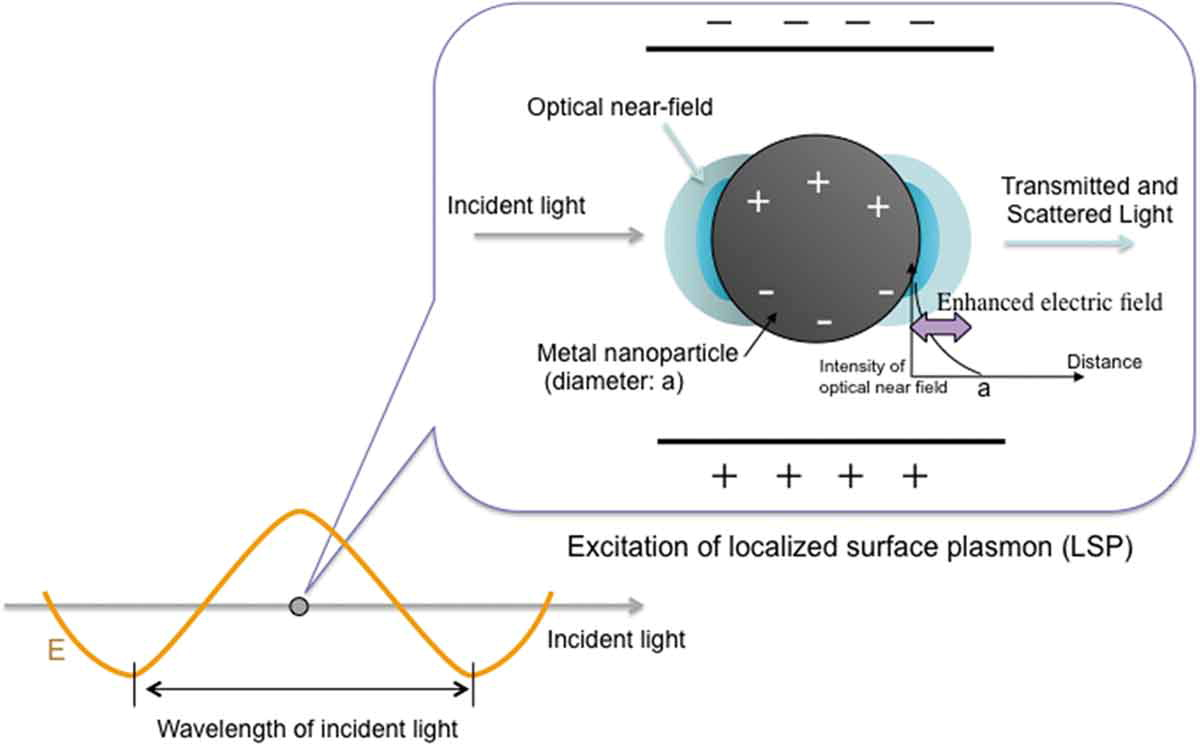
\includegraphics[width=\textwidth]{figures/Theory/E_Field.jpeg}
    \caption{} 
    \label{Fig:EField}
\end{subfigure}
\begin{subfigure}[b]{0.9\textwidth}
    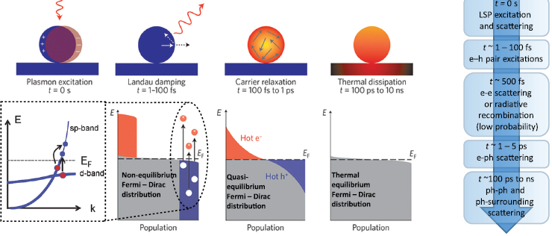
\includegraphics[width=\textwidth]{figures/Theory/Plasmon_Decay.png}
    \caption{}
    \label{Fig:Decay}
    \end{subfigure}
    \caption{Principles of localised surface plasmons (LSPs). (\textbf{a}) How the dipole approximation is manifested, and the origin of LSPs through enhanced local fields. Recreated with permission from \cite{Manzhos2021}. (\textbf{b}) Illustration of the non-radiative decay mode leading to the creation of  pair of hot charge carriers. Recreated with permission from \cite{AuPlasmonRev}.}
    \label{Fig:Plasmonics}
\end{figure}

In Figure \ref{Fig:Plasmonics}, we introduce the origins of plasmonic properties, and demonstrate how their non-equilibrium electron-hole distribution may decay into a pair of hot carriers. In Figure \ref{Fig:EField}, we see the dipole approximation being depicted by a small nanoparticle whose dimensions are far smaller than the wavelength of the light. This is fundamental to the dipole approximation, as it permits us to approximately treat the structure as a perfect dipole oscillator whose modes are described with respect to plasma oscillations - plasmons. Furthermore, in Figure \ref{Fig:Decay}, there is a demonstration of how the plasma oscillations are generated by the $sp$ intraband transitions or the $d$-$sp$ interband transitions, which lead to a non-equilibrium Fermi-Dirac distribution of kinetically active (hot) charge carriers through the mechanism of Landau damping. Within the model described in \cite{AuPlasmonRev}, this hot distribution, these carriers may then begin to relax through scattering and recombination events within the nanostructure if they are not able to be harvested and directed into an adsorbed molecule.

\subsection{Classical Motivation}
\label{sec:class_plasma}

By considering the favourable geometry of a spherical nanoparticle in a uniform electric field, one may derive an expression for the polarisability of the system,

\begin{equation}
    \alpha = 4\pi d^{3}\frac{\varepsilon - \varepsilon_{m}}{\varepsilon + 2\varepsilon_{m}},
    \label{eqn:polarise}
\end{equation}
where $d$ is the radius of the nanoparticle, $\varepsilon_{m}$ is the dielectric constant of the surrounding medium, and $\varepsilon$ is the nanoparticle's dielectric function.

It is indeed from this polarisability that we gain access to measurable and calculable optical properties of our system. Principally, these would be the scattering, $\sigma_{sca}$, absorption, $\sigma_{abs}$, and extinction cross sections, $\sigma_{ext}$ of the specified nanoparticles. With the only necessary assumptions insofar being that the nanoparticle is sufficiently small such that $\lambda >> d$, and that the nanoparticle is indeed spherical, the expressions for such quantities may be given as such:

\begin{equation}
    \sigma_{sca}  = \frac{k^{4}}{6\pi} |\alpha|^{2} = \frac{8\pi}{3}k^{4}d^{6} \left| \frac{\varepsilon - \varepsilon_{m}}{\varepsilon + 2\varepsilon_{m}} \right|^{2},
    \label{eqn:scatter}
\end{equation}

\begin{equation}
\sigma_{abs} = k\Im\left[\alpha\right] = 4\pi k d^{3}\Im\left[ \frac{\varepsilon - \varepsilon_{m}}{\varepsilon + 2\varepsilon_{m}} \right],
\label{eqn:abs}
\end{equation}

\begin{equation}
    \sigma_{ext} = \sigma_{abs} + \sigma_{sca} = 9\frac{\omega}{c}\varepsilon_{m}^{\frac{3}{2}}V \frac{\varepsilon_{\Im}}{\left[ \varepsilon_{\mathbb{R}} + 2\varepsilon_{m} \right]^{2} + \varepsilon_{\Im}^{2}}
    \label{eqn:extinction}
\end{equation}
where $k$ is the wavevector of the incident light, $V$ is the nanoparticle's volume and $c$ is the speed of light in vacuo. Of experimenal interest is the radius scaling relationship between equations \ref{eqn:abs} and \ref{eqn:scatter} in that the former grows as the cube of radius whereas the latter as to the power of 6. The implication here being that it can be difficult to identify small objects in a background of large scatterers. A final point of observation to be made is that one expects both scattering and absorption events to be enhanced at the plasmon resonance frequency.

We now wish to briefly motivate why it is that we require expensive quantum mechanical models for such systems when we have just demonstrated the validity and sufficiency of classical theory. One may consider a specific mechanism which necessitates the incorporation of an explicit quantum model. These classical models discussed above assume a sharp cut-off at the boundary of the nanoparticle, in that all contained charges are bound by the surface. Indeed, this is not the case and is a documented phenomenon known as the electron-density spill-out, or alternatively quantum tunneling effects become profound between clusters \cite{PlasmonTunneling}. As such, size dependent shifts of the main plasmon of isolated nanoparticles or the existence of further surface collective modes that cannot be supported on stepped valence electron distributions are rendered unobtainable via classical models. Moreover, the near-field enhancement of two nanoparticles separated by subnanometer distances cannot be modelled accurately by classical non-local optical models \cite{PlasmonTunneling2}. This is because the physics of such a system features the non-trivial overlap of each constituent nanoparticle's valence electrons permitting the establishment of a photo-induced tunnel current. As we shall discuss in more detail through this report, the quantum mechanical description of sub-nanometric plasma physics may faithfully be captured via density functional theory methods.

\subsection{Quantum Mechanical Description}
\label{sec:quant_plasma}

At the quantum mechanical level of theory, it quickly becomes unclear as to what the origin of an observed excitation may be. In one instance, it may indeed be the result of a collective oscillation of the metal's valence electrons, hence being correctly identified as an LSP. However; it may also be the case that an observed peak in the absorption spectrum of a cluster is the result of a single electron - hole pair excitation. These are less desirable to generate in a cluster as they will typically recombine monotonically. Whereas we are instead interested in the Landau damping of an LSP which causes the collective oscillation to decay into a pair of hot carriers \cite{ExtractHotCars}. Until recently, there have been few viable means of discriminating between the two types of excitation \cite{PhotoExcited}. There have existed several which are theory specific, however these have lacked generality and transferability. Recently, there has been proposed a generalised plasmonicity index (GPI) \cite{GPI}, which intends to resolve this very issue by considering the relative ratio between the induced field enhancement of a nanoparticle, and the applied external field. At present, this method has been tested in the classical Mie theory and in the random phase approximation (RPA)\footnote{The RPA is an alternative method of computing quantum mechanical electronic interactions which was developed in the 50's by Davids Bohm and Pines \cite{RPA1,RPA2,RPA3} and is an established method for describing plasma oscillations in MNPs \cite{doi:10.1143/JPSJ.80.044606}.}, showing promise. Throughout this project, we intend to assess the plasmonicity of our structures for reasons discussed above. 

We are explicitly interested in plasmonic materials given the non-radiative decay mode of localised surface plasmons into a pair of hot carriers via the process of Landau damping, as seen in Figure \ref{Fig:Decay}, which may then be used to facilitate the catalysis of chemical reactions such as water splitting \cite{LSPCatalysis}. We may excite these carriers optically by first exciting the target metal at its plasma frequency. Following  optical excitation, electrons in a plasmonic metal, a non-equilibrium step-like hot-electron distribution is formed in the energy range around the Fermi level. For smaller objects, one may more accurately describe the Fermi level as the highest occupied molecular orbital (HOMO) as within finite systems one lacks the periodicity necessary to form a Fermi surface. In the common description of hot-electron relaxation in plasmonic metals \cite{PhysRevB.50.15337,PhysRevB.100.045412,Sjakste_2018,doi:10.1021/acsphotonics.7b00751,Memarzadeh:20,osti_1594820}, this non-equilibrium population decays within the first few hundred femtoseconds due to a sequence of elastic electron~-~electron collisions resulting in the equilibrium population of electrons with the temperature higher than the background ionic temperature. These thermalised hot electrons cool down with emission of phonons, and through vibrational modes in finite systems. 

As discussed above, the field of research regarding photo-catalysis on nanoparticles alone is vast and while we do not wish for this to become a review article, it is only appropriate to discuss recent contributions which have profoundly moulded the direction taken within this project. In principle, we shall discuss a wide range of techniques employed to model the hot carrier creation and transfer on a nanoparticle's surface \cite{NordLander,HotCarrierTransport}, advanced sampling techniques for finding thermodynamically stable clusters \cite{Structure_Thermo_EnergyLandscape,FerrandoEquilibrium}, and the growing trend in employing machine learning techniques in the development of atomistic forcefields \cite{MLInterface,hansen2019atomisticMLFF}.

While it is well established that there must be a hot carrier transfer process from catalyst to molecule, it remains a point of active research in myriad communities how the transfer process may manifest \cite{Furube2017}. Indeed, this property is studied beyond the realm of plasmon enhanced photo-catalysis, and is pertinent to the biological communities \cite{Giannini2019} where charge transfer mechanisms are understood to be significant to comprehensively understanding cellular activity \cite{doi:10.1021/acs.chemrev.5b00298}. Moreover, it is often difficult to determine whether or not charge has been transferred directly, in that an electron from within the Fermi sea of the catalyst may be transferred to an unoccupied state of the adsorbed molecule - or vice versa. This is known to be a more efficient charge transfer mechanism that that of indirect transfer, in which an electron - hole pair is created within the catalyst and then a hot carrier is transferred to the molecule. This is inherently less efficient as it is more likely that the hot carrier pair will recombine in this regime. To study this effect at the atomistic scale, a recent paper has been published in which a single CO molecule had been adsorbed onto one of three unique bonding sites of an Ag$_{147}$ nanoparticle \cite{AuTRansfer}. It was determined that the geometry of the adsorption site was significant in promoting the direct charge transfer mechanism. From this study, we may follow a similar line of questioning to determine how best to adsorb water onto the surfaces of our composite AuPt nanoparticles.


